\documentclass[10pt]{beamer}
% Introduction to Control and Machine Learning: the opening lecture of the course.
% Converted from the PowerPoint deck slides-master-part1 (E. Zuazua, October 2026).
% The videos of the original deck are not embedded: each video slide shows a still
% frame that links to the source on YouTube or, for the four clips that have no
% public source, to the small copies in videos/ served by the course website.

\usepackage[T1]{fontenc}
\usepackage[utf8]{inputenc}

\usetheme{metropolis}
\metroset{sectionpage=none}

\usepackage{graphicx}
\graphicspath{{images/}}
\usepackage{amsmath, amssymb}
\usepackage{bm}
\usepackage{array}
\usepackage{tikz}
\usetikzlibrary{positioning, arrows.meta, calc}
\usepackage{xcolor}
\usepackage[most]{tcolorbox}
\definecolor{boxbg}{RGB}{235,245,255}
\definecolor{boxframe}{RGB}{70,130,180}
\definecolor{questbg}{RGB}{253,236,232}
\definecolor{questframe}{RGB}{170,40,30}
\definecolor{ctrl}{HTML}{EB6834}    % P.ORANGE: the control, as in the figures of lecture 01
\definecolor{param}{HTML}{1F4FBF}   % the parameters that are learned
\definecolor{act}{HTML}{C83030}     % the activation function

\hypersetup{colorlinks=true, linkcolor=., urlcolor=boxframe}

\title{Introduction to Control and Machine Learning}
\subtitle{Mathematical Foundations of Control and Machine Learning}
\author{Enrique Zuazua}
\date{Winter 2026}
\institute{FAU Erlangen-N\"urnberg}

% --- Math shortcuts --------------------------------------------------------
\newcommand{\R}{\mathbb{R}}
\newcommand{\ctrl}[1]{\textcolor{ctrl}{#1}}
\newcommand{\param}[1]{\textcolor{param}{#1}}
\newcommand{\act}[1]{\textcolor{act}{#1}}
\DeclareMathOperator{\rank}{rank}

% --- Boxes -----------------------------------------------------------------
\newtcolorbox{mathbox}[2][]{
  colback=boxbg, colframe=boxframe, boxrule=0.2pt, arc=2pt,
  left=4pt, right=4pt, top=2pt, bottom=2pt,
  title=\textbf{#2}, fonttitle=\small, coltitle=white, colbacktitle=boxframe,
  halign=left, #1}
\newtcolorbox{questionbox}{
  colback=questbg, colframe=questframe, boxrule=0.2pt, arc=2pt,
  left=4pt, right=4pt, top=3pt, bottom=3pt, halign=center}

% --- Pictures and videos ---------------------------------------------------
% \fitimg[fraction]{file}: an image as large as the frame allows.
\newcommand{\fitimg}[2][0.8]{\includegraphics[width=\textwidth, height=#1\textheight, keepaspectratio]{#2}}
% \caption*: a one-line caption under a picture.
\newcommand{\picnote}[1]{{\par\smallskip\scriptsize\color{black!60}#1\par}}
% \videoframe{graphics options}{poster}{url}{caption}: a still frame of a video;
% both the frame and the caption open the video in the browser.
\newcommand{\videoframe}[4]{%
  \begin{center}
  \href{#3}{\includegraphics[#1]{#2}}\par\smallskip
  {\scriptsize\href{#3}{$\blacktriangleright$\ #4}\par}
  \end{center}}

\setbeamerfont{standout}{size=\Large, series=\mdseries}

\begin{document}

\maketitle

% =========================================================================
\begin{frame}{Plan of the lecture}
\begin{enumerate}
\item \alert{The context today.} Artificial intelligence everywhere: in science, in the economy, in what we see; representation, and the risk of hallucinations.
\item \alert{Origins.} Aristotle; Watt's governor and Maxwell; Wiener's cybernetics and Kalman's theorem; Markov chains and PageRank; herding and parking.
\item \alert{Machine learning objectives.} Express and represent, generalize and forecast, generate and create. Universal approximation, shallow and deep networks, supervised learning, least squares, sampling.
\item \alert{Video material.} The 3Blue1Brown series on neural networks.
\end{enumerate}

\bigskip
\small
Notebook \textbf{00} of the course, \emph{The Big Picture: Control and Machine Learning}, complements these slides. The videos of the lecture are not embedded in this PDF: click on a still frame to open the video. The original PowerPoint, with the videos embedded, is on \href{https://drive.google.com/file/d/1iTSIfdrd_4o3Lwf-c-V_9y__BtAXT8Vc/view}{Google Drive} (300\,MB).
\end{frame}


% =========================================================================
\section{The context today}

\begin{frame}[standout]
The context today
\end{frame}


\begin{frame}[plain]
\begin{columns}[c]
\begin{column}{0.5\textwidth}
\centering

\includegraphics[width=0.85\linewidth]{ai_letters}
\end{column}
\begin{column}{0.45\textwidth}
\visible<2>{%
\small Two letters, many meanings:
\begin{itemize}\setlength{\itemsep}{0pt}
\item Adobe Illustrator
\item Artificial Insemination
\item Aortic Insufficiency
\item Academic Integrity
\item All Inclusive
\item Automotive Industry
\item Aviation Insurance
\item Area of Interest
\item Annual Income
\item Air India
\end{itemize}}
\end{column}
\end{columns}
\end{frame}


\begin{frame}[plain]
\begin{tikzpicture}[remember picture, overlay]
  \node at (current page.center) {
\includegraphics[width=4cm]{ai_letters}};
  \node[anchor=north west] at ([xshift=14mm, yshift=-12mm] current page.north west) {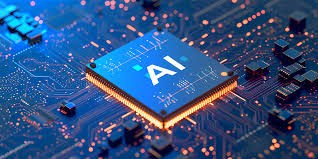
\includegraphics[width=3.4cm]{ai_chip}};
  \node[anchor=north east] at ([xshift=-14mm, yshift=-12mm] current page.north east) {
\includegraphics[width=2.8cm]{ai_circuit_icon}};
  \node[anchor=south west] at ([xshift=14mm, yshift=12mm] current page.south west) {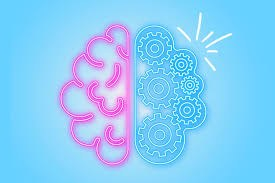
\includegraphics[width=3.4cm]{ai_brain_gears}};
  \node[anchor=south east] at ([xshift=-14mm, yshift=12mm] current page.south east) {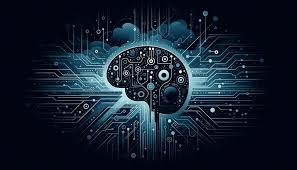
\includegraphics[width=3.4cm]{ai_brain_dark}};
\end{tikzpicture}
\end{frame}


% =========================================================================
\begin{frame}{The ubiquity of AI in science}
\begin{columns}[T]
\begin{column}{0.56\textwidth}
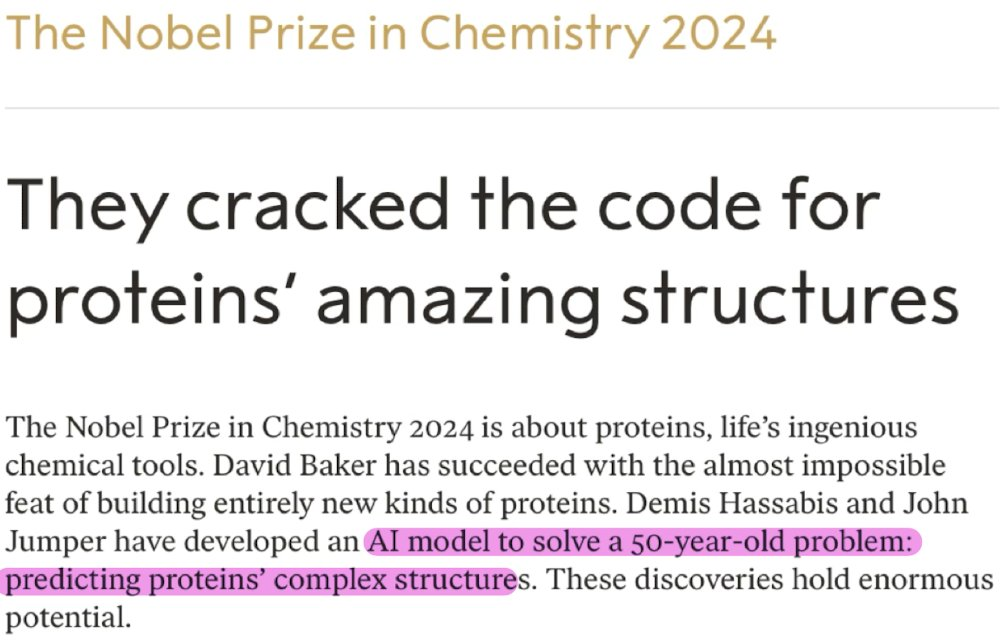
\includegraphics[width=\linewidth]{nobel_chemistry_2024}

\smallskip
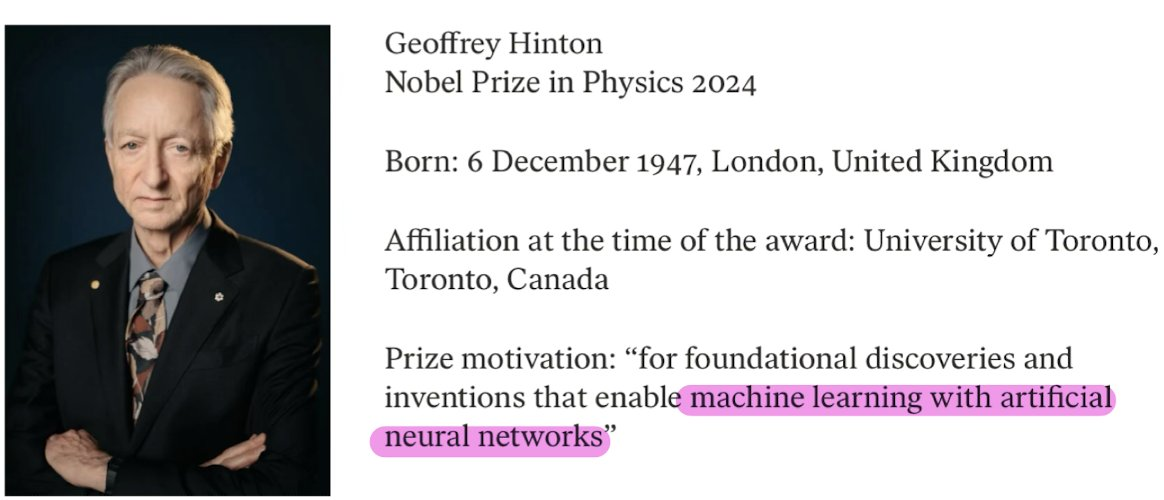
\includegraphics[width=\linewidth]{hinton_nobel_physics_2024}
\end{column}
\begin{column}{0.4\textwidth}
\vspace{1.4cm}

\includegraphics[width=\linewidth]{deepseek_chatgpt}

\medskip
\footnotesize
The 2024 Nobel Prizes in Chemistry (Baker, Hassabis, Jumper) and Physics (Hopfield, Hinton) reward machine learning: protein structure prediction and the foundations of artificial neural networks.
\end{column}
\end{columns}
\end{frame}


\begin{frame}[plain]
\centering

\includegraphics[width=\textwidth]{its_a_bubble_cartoon}
\end{frame}


% =========================================================================
\begin{frame}{This person does not exist}
\centering
\href{https://this-person-does-not-exist.com}{\fitimg[0.78]{this_person_does_not_exist}}
\picnote{A face generated by a neural network: \href{https://this-person-does-not-exist.com}{this-person-does-not-exist.com}.}
\end{frame}


\begin{frame}{A computer animated hand, 1972}
\centering
\href{https://en.wikipedia.org/wiki/A_Computer_Animated_Hand}{\fitimg[0.76]{wikipedia_computer_animated_hand}}
\picnote{E. Catmull and F. Parke digitize a hand with 350 polygons. \href{https://en.wikipedia.org/wiki/A_Computer_Animated_Hand}{Wikipedia: \emph{A Computer Animated Hand}.}}
\end{frame}


\begin{frame}[plain]
\begin{columns}[c]
\begin{column}{0.5\textwidth}
\centering
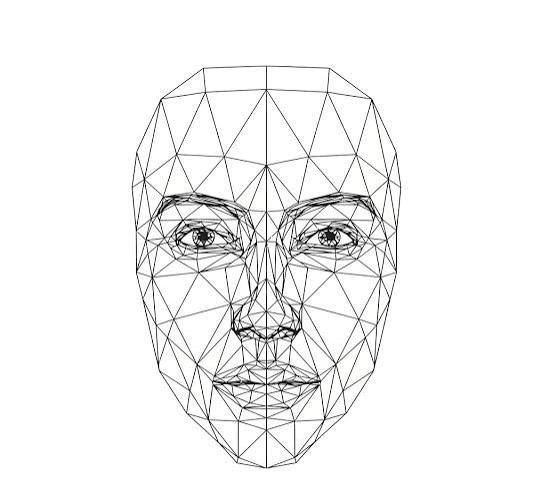
\includegraphics[width=0.92\linewidth, height=0.72\textheight, keepaspectratio]{face_wireframe}
\end{column}
\begin{column}{0.5\textwidth}
\centering
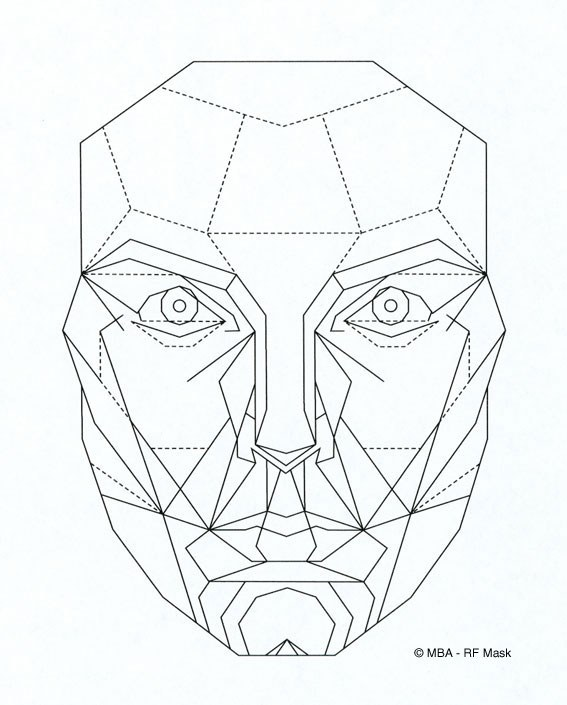
\includegraphics[width=0.92\linewidth, height=0.72\textheight, keepaspectratio]{face_mask_mba}
\end{column}
\end{columns}
\end{frame}


\begin{frame}{Representing a surface: Tutte embeddings}
\centering
\href{https://www.gpeyre.com/mathematical-nexus/}{\fitimg[0.6]{peyre_tutte_embedding}}
\picnote{Tutte's theorem (1963) draws a planar graph by solving a linear system; it is the basis of surface parameterization in mesh processing. Gabriel Peyré, \href{https://www.gpeyre.com/mathematical-nexus/}{Mathematical Nexus}.}
\end{frame}


\begin{frame}{Discrete differential geometry}
\centering
\href{https://www.cs.cmu.edu/~kmcrane/}{\fitimg[0.72]{keenan_crane_webpage}}
\picnote{\href{https://www.cs.cmu.edu/~kmcrane/}{Keenan Crane, Carnegie Mellon University}: geometry processing, Monte Carlo methods for PDEs.}
\end{frame}


% =========================================================================
\begin{frame}{The risk of hallucinations}
\centering
\fitimg[0.82]{hallucinating_robot}
\end{frame}


\begin{frame}{Real or AI?}
\videoframe{height=0.72\textheight}{poster_real_or_ai}{https://www.youtube.com/shorts/3Rf2bizgG-M}{ABC News (Australia): \emph{Is it real or AI? It's getting harder than ever to tell the difference} (video, 3 min)}
\end{frame}


\begin{frame}{The risk of hallucinations}
\centering
\fitimg[0.76]{dali_temptation_st_anthony}
\picnote{Salvador Dalí, \emph{The Temptation of Saint Anthony} (1946).}
\end{frame}


\begin{frame}[plain]
\centering
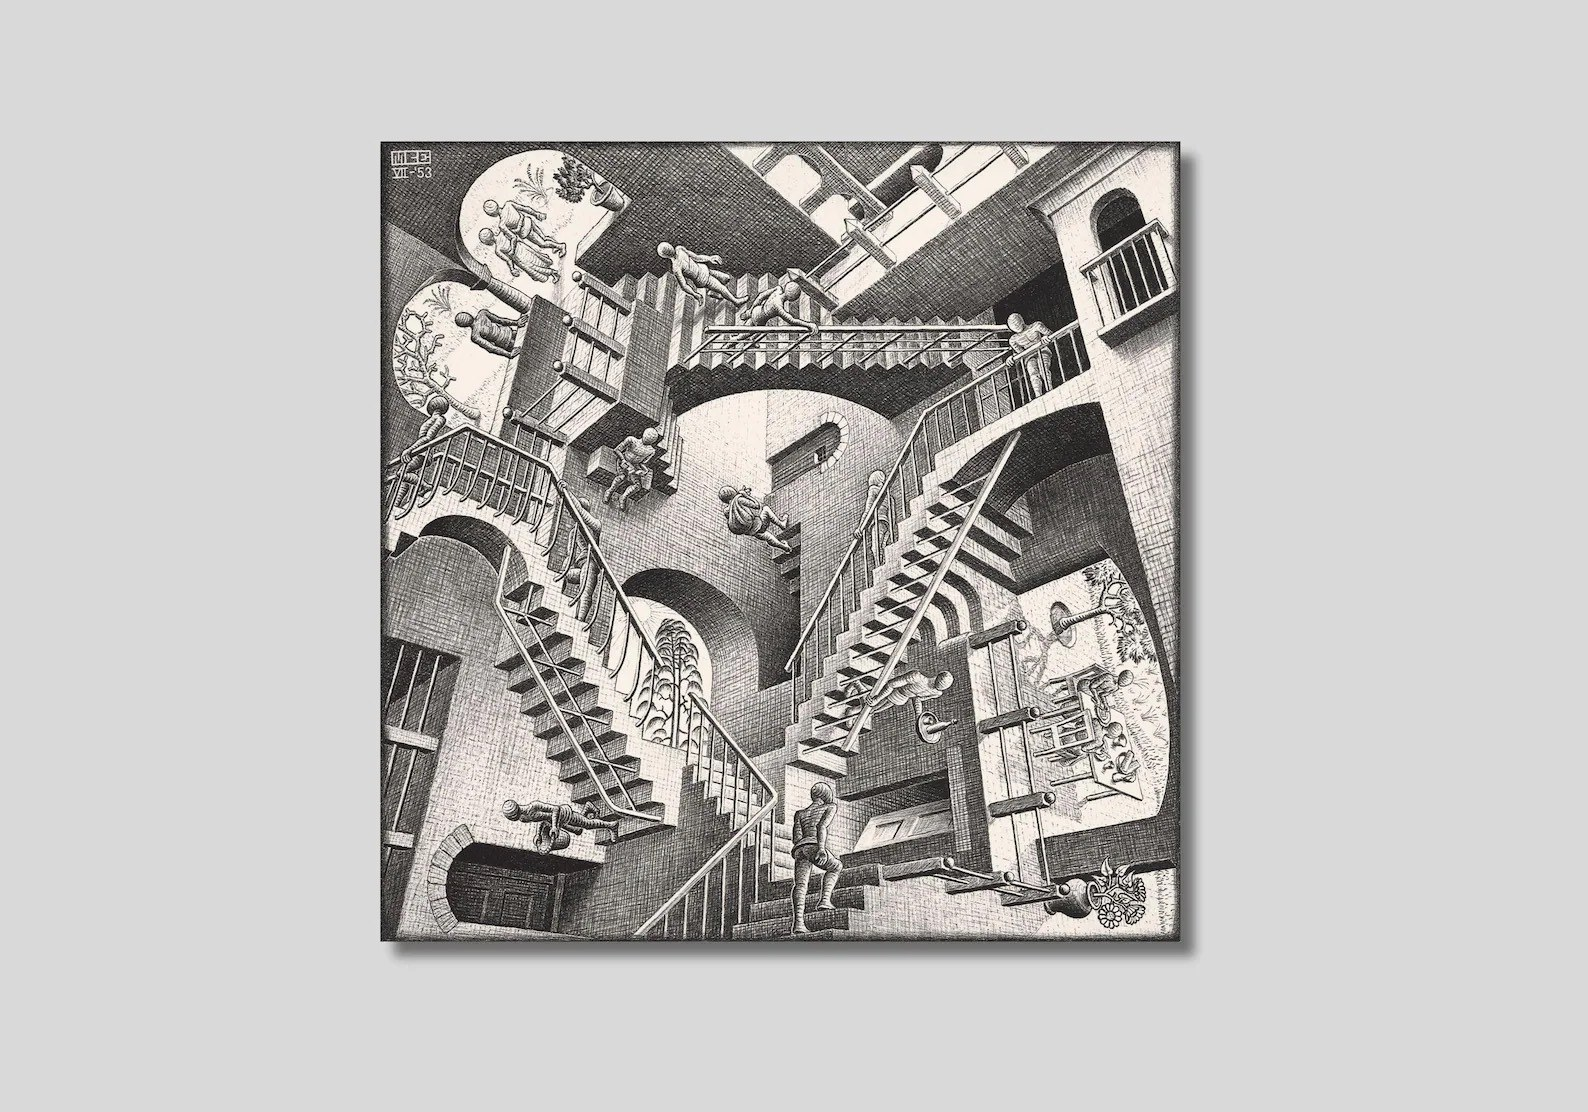
\includegraphics[height=0.8\textheight, width=\textwidth, keepaspectratio]{escher_relativity}
\picnote{M. C. Escher, \emph{Relativity} (1953).}
\end{frame}


\begin{frame}[plain]
\centering
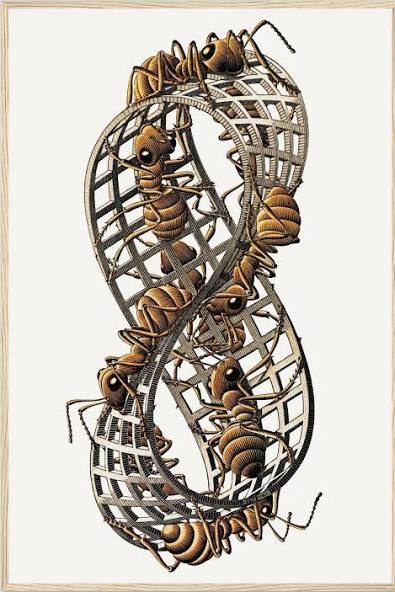
\includegraphics[height=0.8\textheight]{escher_moebius_strip_ii}
\picnote{M. C. Escher, \emph{Möbius Strip II} (1963).}
\end{frame}


\begin{frame}[plain]
\centering
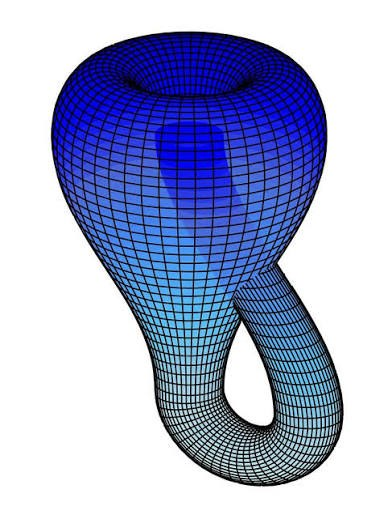
\includegraphics[height=0.78\textheight]{klein_bottle}
\picnote{The Klein bottle. Felix Klein was professor in Erlangen (1872--1875), where he formulated the Erlangen program.}
\end{frame}


% =========================================================================
\section{Origins}

\begin{frame}[standout]
Origins
\end{frame}


\begin{frame}[plain]
\vfill
\centering
\Large
When did artificial intelligence emerge, or when did the race toward what we now call artificial intelligence begin?
\vfill
\end{frame}


\begin{frame}{Aristotle}
\begin{columns}[c]
\begin{column}{0.72\textwidth}
\small\itshape
``If every instrument could accomplish its own work, obeying or anticipating the will of others, like the statues of Daedalus or the tripods of Hephaestus\ldots\ then master-craftsmen would have no need of assistants, and masters no need of slaves.''

\medskip
\upshape\hfill --- Aristotle, \emph{Politics}, Book I, Ch.~4 (335--323 BC)
\end{column}
\begin{column}{0.24\textwidth}
\centering
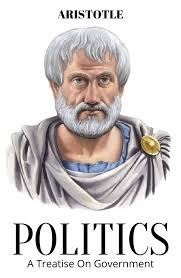
\includegraphics[width=0.85\linewidth]{aristotle_politics_cover}
\end{column}
\end{columns}

\pause
\medskip
\small
\begin{itemize}
\item \alert{Automation.} He imagined a world where tools (instruments) could perform tasks autonomously, anticipating or obeying commands.
\item \alert{Liberation from labor.} This automation would eliminate the need for human labor, freeing people from mundane work.
\item \alert{Relevance today.} Aristotle's thought experiment foreshadows modern discussions on automation, robotics and artificial intelligence.
\end{itemize}
\end{frame}


\begin{frame}[plain]
\centering
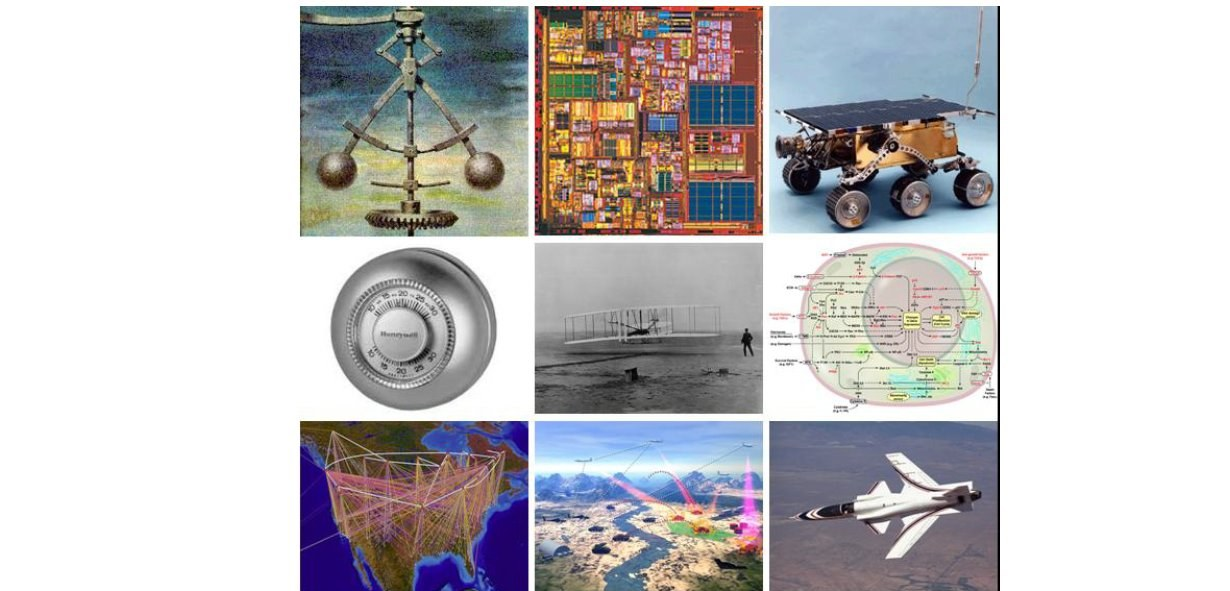
\includegraphics[height=0.78\textheight, width=\textwidth, keepaspectratio]{murray_2003_control_collage}
\picnote{\emph{Control in an Information Rich World}, SIAM, R. Murray (ed.), 2003.}
\end{frame}


% =========================================================================
\begin{frame}{Maxwell, 1868: \emph{On Governors}}
\centering
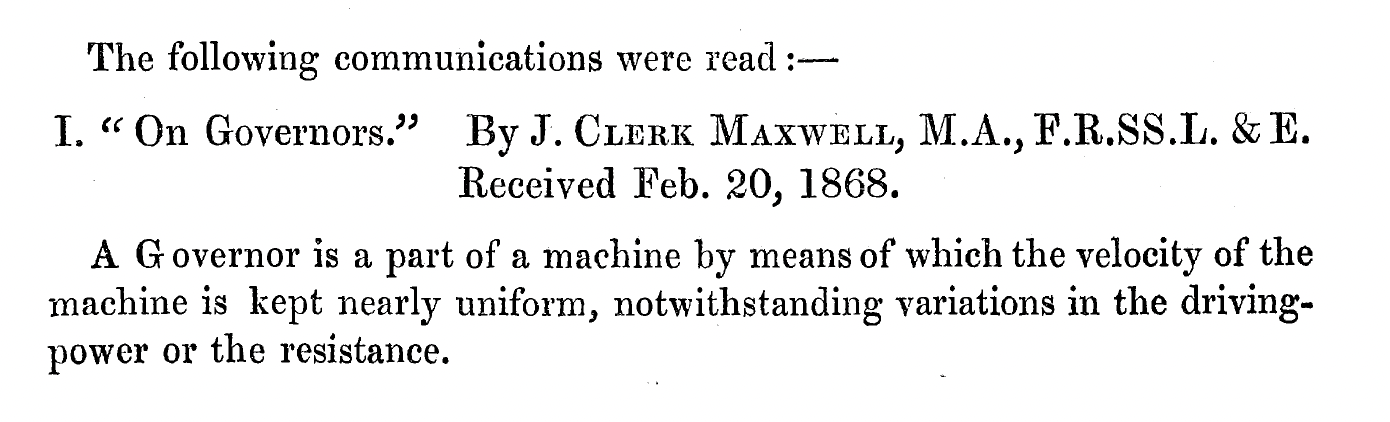
\includegraphics[width=0.94\textwidth]{maxwell_on_governors_text}

\medskip
\begin{columns}[c]
\begin{column}{0.42\textwidth}
\centering
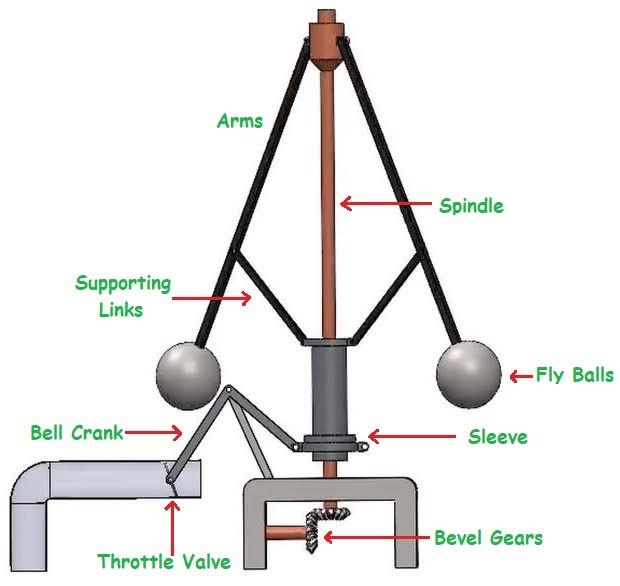
\includegraphics[height=4cm]{centrifugal_governor_diagram}
\end{column}
\begin{column}{0.54\textwidth}
\centering
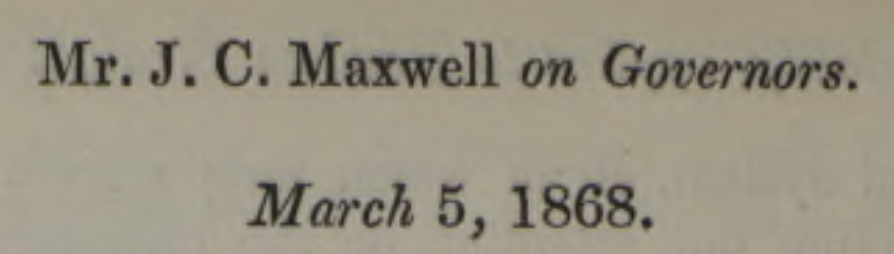
\includegraphics[width=0.9\linewidth]{maxwell_on_governors_header}

\medskip
\footnotesize
Watt's centrifugal governor (1788) keeps the speed of a steam engine nearly uniform. Maxwell asks when such a feedback device settles and when it oscillates: the first stability analysis.

\smallskip
\scriptsize \href{https://webhomes.maths.ed.ac.uk/~v1ranick/papers/maxwell1.pdf}{J. C. Maxwell, \emph{On Governors}, Proc. Royal Society of London 16 (1868), 270--283.}
\end{column}
\end{columns}
\end{frame}


\begin{frame}[plain]
\begin{tikzpicture}[remember picture, overlay]
  \node[anchor=north west] at ([xshift=10mm, yshift=-8mm] current page.north west) {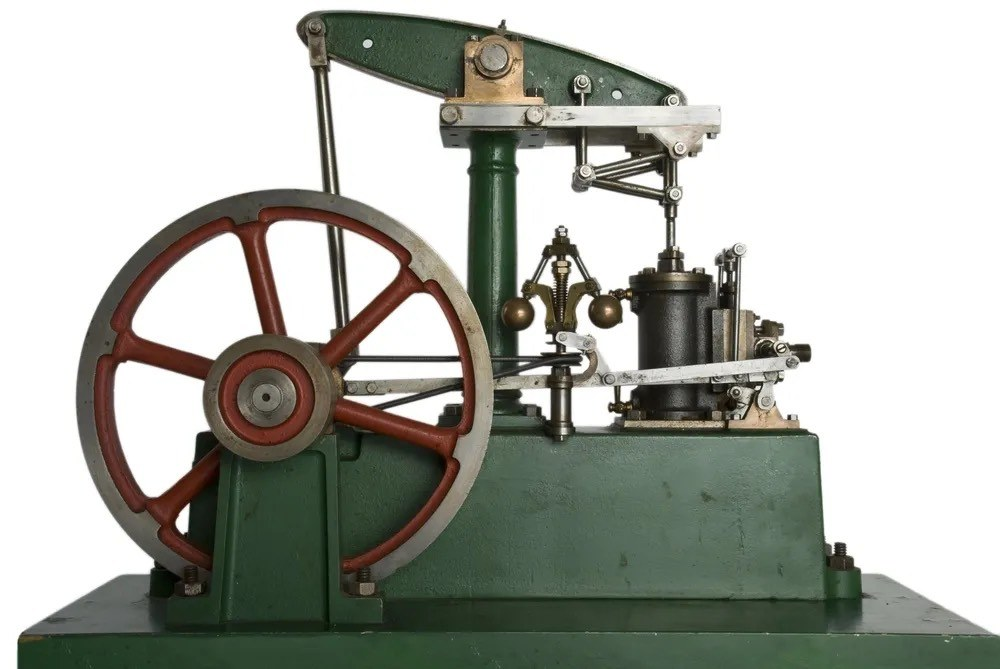
\includegraphics[width=5.2cm]{steam_engine}};
  \node at ([yshift=2mm] current page.center) {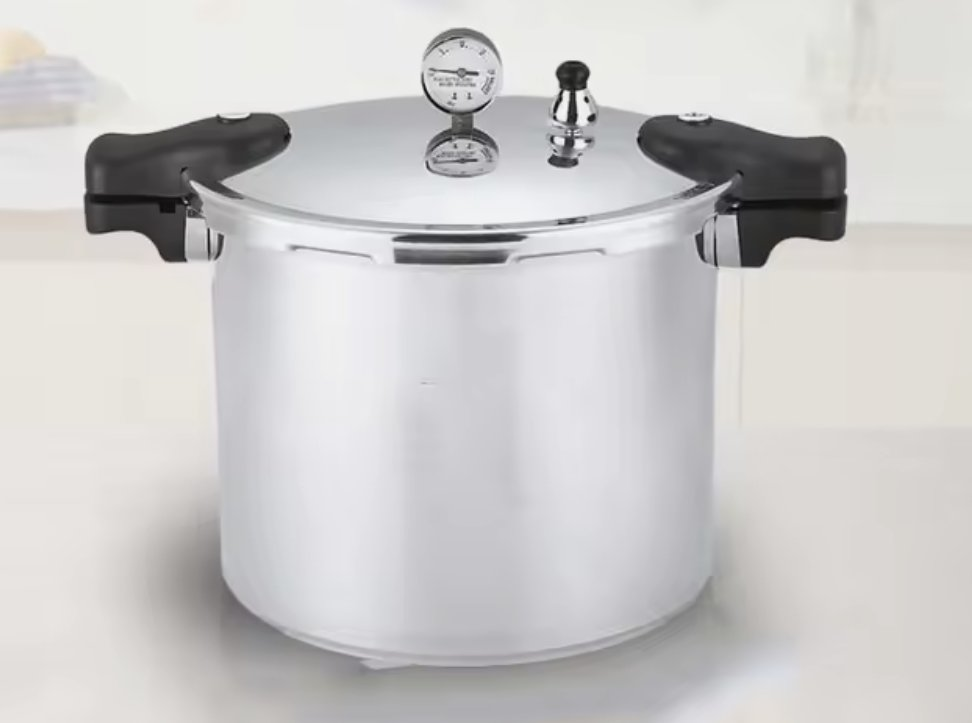
\includegraphics[width=5.4cm]{steam_locomotive}};
  \node[anchor=south east] at ([xshift=-10mm, yshift=8mm] current page.south east) {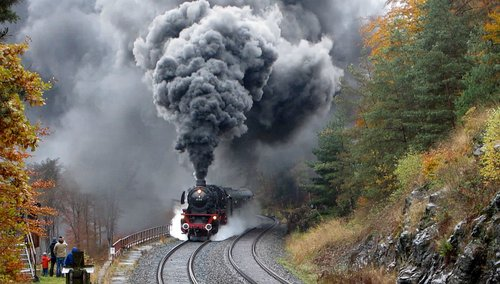
\includegraphics[width=4.6cm]{pressure_cooker}};
\end{tikzpicture}
\end{frame}


% =========================================================================
\begin{frame}{Cybernetics, Norbert Wiener, 1948}
\framesubtitle{The science of control and communication in animals and machines}
\begin{tikzpicture}[remember picture, overlay]
  \node[anchor=north east] at ([xshift=-3mm, yshift=-1.5mm] current page.north east) {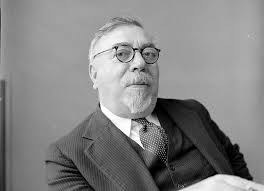
\includegraphics[height=1.55cm]{wiener}};
\end{tikzpicture}
\small
The linear finite $d$-dimensional system
\[
x'(t) = A\,x(t) + \ctrl{B\,u(t)}, \quad t\in(0,T); \qquad x(0) = x^0, \tag{1}
\]
with $m \ll d$ controls. $A\in M_{d\times d}$, $B\in M_{d\times m}$ and $x^0\in\R^d$; $x:[0,T]\to\R^d$ represents the \alert{state} and $u:[0,T]\to\R^m$ the \ctrl{control}.

\begin{questionbox}
Can we control $d$ states with only $m$ controls, even if $d \gg m$?
\end{questionbox}

\begin{columns}[c]
\begin{column}{0.78\textwidth}
\begin{mathbox}{Theorem (R. E. Kálmán, 1960)}
System (1) is controllable if and only if
\[
\rank\,[\,B,\ AB,\ \cdots,\ A^{d-1}B\,] = d.
\]
\end{mathbox}
\end{column}
\begin{column}{0.2\textwidth}
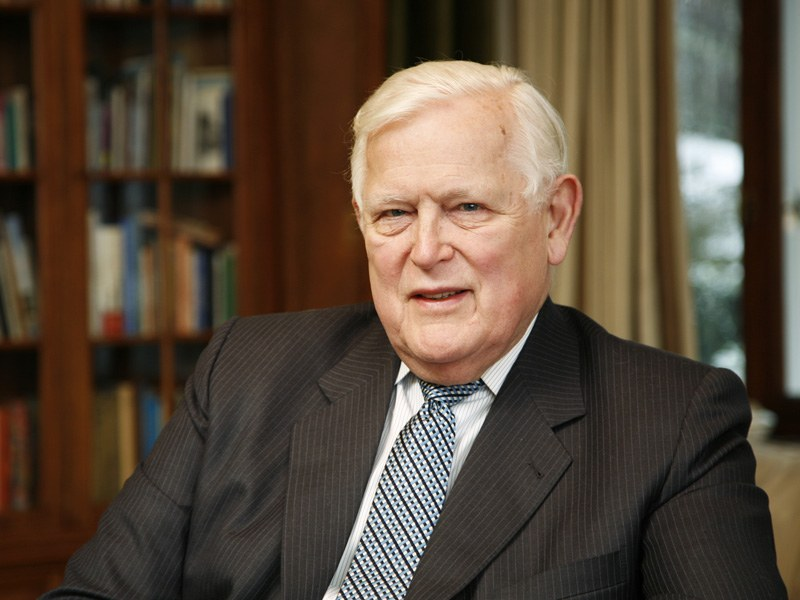
\includegraphics[width=\linewidth]{kalman}
\end{column}
\end{columns}
\end{frame}


% =========================================================================
\begin{frame}{A new paradigm: mathematics + artificial intelligence}
\small
\alert{PageRank}: Larry Page and Sergey Brin (Google, 1998). The importance of a web page is the stationary distribution of a random walk on the graph of links.

\medskip
\centering
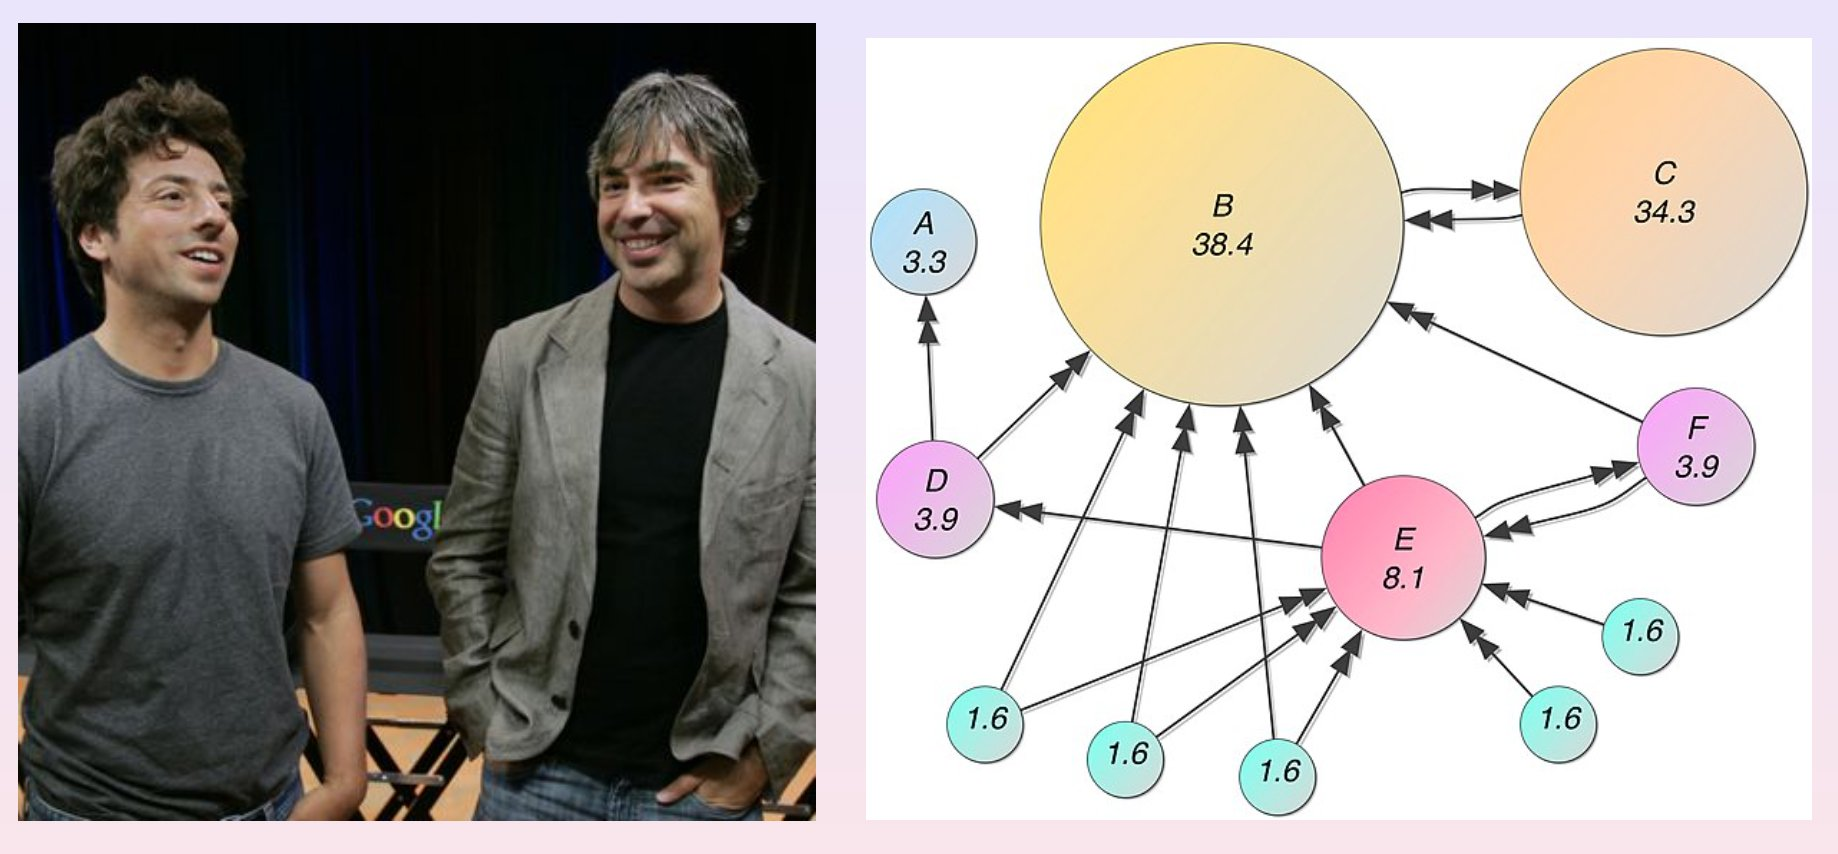
\includegraphics[width=0.92\textwidth]{pagerank_page_brin}

\medskip
\small
Inspired on the \alert{Perron--Frobenius theorem}: Oskar Perron (1880--1975), Georg Frobenius (1849--1917).
\end{frame}


\begin{frame}{Andrey Markov (1856--1922)}
\begin{columns}[c]
\begin{column}{0.58\textwidth}
\small
\begin{itemize}
\item Born 14 June 1856 in Ryazan; died 20 July 1922 in Petrograd. St.\ Petersburg University.
\item Known for \alert{Markov chains} and \alert{Markov processes}: random sequences in which the next state depends only on the present one.
\item Markov chains are the mathematics behind PageRank and the simplest example of a stochastic dynamical system (lecture 01).
\end{itemize}
\smallskip
\scriptsize \href{https://en.wikipedia.org/wiki/Andrey_Markov}{Wikipedia: Andrey Markov.}
\end{column}
\begin{column}{0.4\textwidth}
\centering
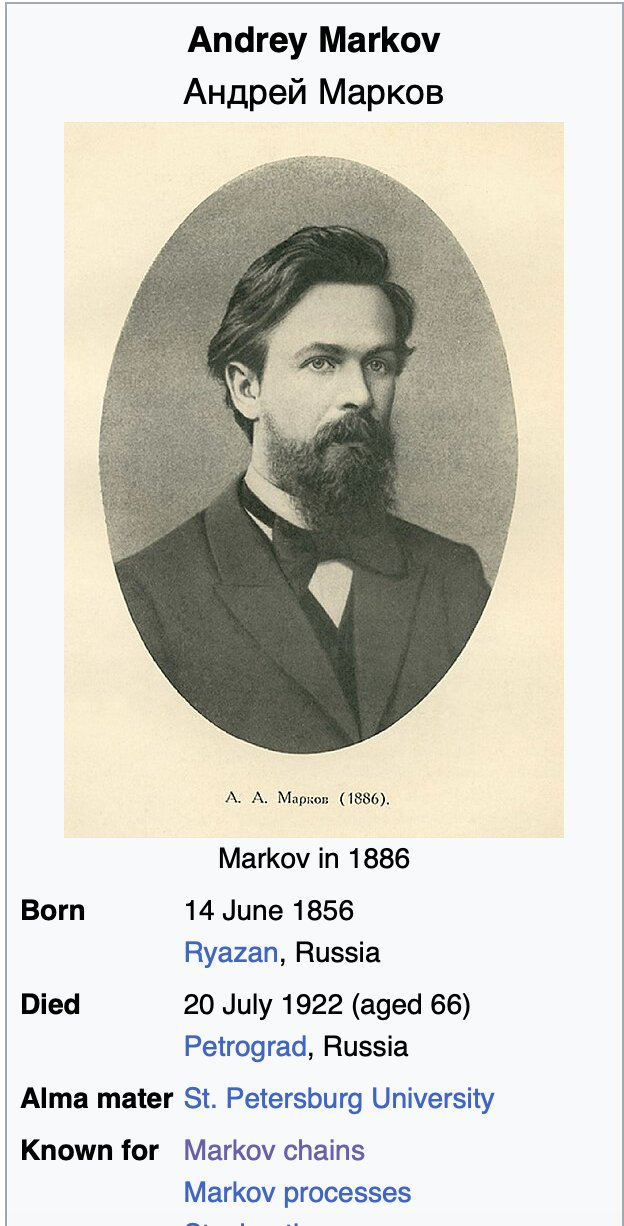
\includegraphics[height=0.82\textheight]{markov_wikipedia_infobox}
\end{column}
\end{columns}
\end{frame}


\begin{frame}{Video: introduction to Markov chains}
\videoframe{width=0.86\textwidth}{poster_markov_chains}{https://www.youtube.com/watch?v=i3AkTO9HLXo}{Normalized Nerd: \emph{Markov Chains Clearly Explained! Part 1} (video, 9 min)}
\end{frame}


\begin{frame}{Video: Google's algorithm through Markov chains}
\videoframe{width=0.86\textwidth}{poster_pagerank}{https://www.youtube.com/watch?v=JGQe4kiPnrU}{Reducible: \emph{PageRank: A Trillion Dollar Algorithm} (video, 25 min)}
\end{frame}


% =========================================================================
\begin{frame}[plain]
\centering

\includegraphics[height=0.92\textheight]{hairer_wanner_cover}
\end{frame}


\begin{frame}{Analysis by its history}
\footnotesize
\begin{quote}
\ldots\ I should like to bring up again for emphasis \ldots\ points, in which my exposition differs especially from the customary presentation in the textbooks:
1.~Illustration of abstract considerations by means of figures.
2.~Emphasis upon its relation to neighboring fields, such as calculus of differences and interpolation\ldots\
3.~Emphasis upon historical growth.
It seems to me extremely important that precisely the prospective teacher should take account of all of these. \hfill (F. Klein 1908, Engl.\ ed.\ p.~236)
\end{quote}

\small
Traditionally, a rigorous first course in Analysis progresses (more or less) in the following order:
\[
\text{sets, mappings} \;\Rightarrow\; \text{limits, continuous functions} \;\Rightarrow\; \text{derivatives} \;\Rightarrow\; \text{integration.}
\]
On the other hand, the historical development of these subjects occurred in reverse order:
\[
\begin{array}{c}\text{Cantor 1875}\\ \text{Dedekind}\end{array}
\;\Leftarrow\;
\begin{array}{c}\text{Cauchy 1821}\\ \text{Weierstrass}\end{array}
\;\Leftarrow\;
\begin{array}{c}\text{Newton 1665}\\ \text{Leibniz 1675}\end{array}
\;\Leftarrow\;
\begin{array}{c}\text{Archimedes}\\ \text{Kepler 1615}\\ \text{Fermat 1638}\end{array}
\]
\scriptsize E. Hairer and G. Wanner, \emph{Analysis by Its History}, Undergraduate Texts in Mathematics, Springer, 1996 (preface).
\end{frame}


% =========================================================================
\begin{frame}{True herding}
\videoframe{width=0.8\textwidth}{poster_sheepdog_trial}{https://cml-fau.github.io/lectures/00_introduction_control_and_machine_learning/videos/sheepdog_trial.mp4}{A sheepdog trial: the shepherd steers the flock through the dog (video, 1:51)}
\end{frame}


\begin{frame}{Robotic herding}
\videoframe{height=0.72\textheight}{poster_robot_dog}{https://www.youtube.com/shorts/4NxzqaRJh6U}{University of the Sunshine Coast: \emph{Robotic dog herding sheep in regional Queensland} (video, 15 s)}
\end{frame}


\begin{frame}{Virtual herding}
\videoframe{height=0.74\textheight}{poster_virtual_herding}{https://cml-fau.github.io/lectures/00_introduction_control_and_machine_learning/videos/virtual_herding.mp4}{Simulation: one controlled agent (red) drives the flock (yellow) into the pen (video, 20 s)}
\end{frame}


\begin{frame}{An example: Nelson's car}
\begin{columns}[c]
\begin{column}{0.5\textwidth}
\videoframe{width=0.9\linewidth}{poster_nelsons_car}{https://cml-fau.github.io/lectures/00_introduction_control_and_machine_learning/videos/nelsons_car.mp4}{Parallel parking (simulation, 40 s)}
\end{column}
\begin{column}{0.46\textwidth}
\centering
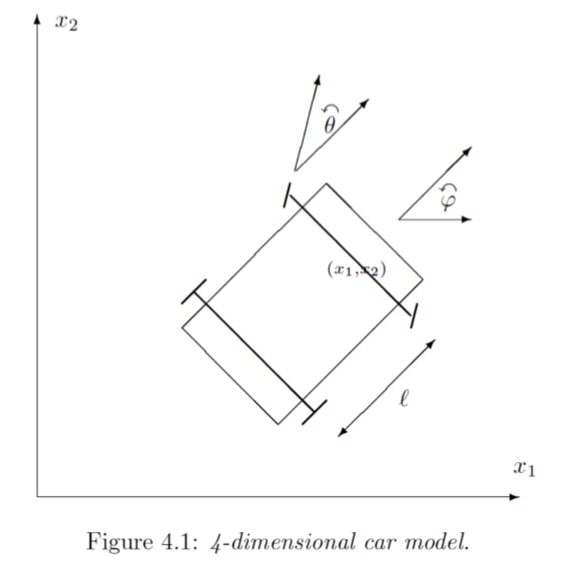
\includegraphics[width=0.78\linewidth]{nelson_car_model_sontag}
\end{column}
\end{columns}

\footnotesize
The state is four-dimensional, position $(x_1,x_2)$, orientation $\theta$ and steering angle $\varphi$, and there are two controls, the speed and the rotation of the wheel.
\alert{Two controls suffice to control a four-dimensional dynamical system.}

\smallskip
\scriptsize E. Sontag, \emph{Mathematical Control Theory}, 2nd ed., Springer-Verlag, New York, 1998, Figure 4.1.
\end{frame}


\begin{frame}[plain]
\videoframe{height=0.84\textheight}{poster_car_parking}{https://cml-fau.github.io/lectures/00_introduction_control_and_machine_learning/videos/car_parking.mp4}{Automatic parking (video, 30 s)}
\end{frame}


% =========================================================================
\section{Machine learning objectives}

\begin{frame}[standout]
Machine learning objectives
\end{frame}


\begin{frame}{ML objectives}
\vfill
\Large
\begin{itemize}
\setlength{\itemsep}{1.6em}
\item \textbf{Express / Represent}
\item \textbf{Generalize / Forecast}
\item \textbf{Generate / Create}
\end{itemize}
\vfill
\end{frame}


\begin{frame}[standout]
Express / Represent
\end{frame}


% =========================================================================
\begin{frame}{Why does it work? Universal approximation}
\begin{columns}[T]
\begin{column}{0.62\textwidth}
\small
\textbf{N. Wiener}, Tauberian theorems, \emph{Annals of Mathematics} 33 (1) (\textbf{1932}), 1--100.
\[
f(x) \sim \sum_{j=1}^{K} \param{w_j}\, \act{G}(x + \param{b_j})
\]

\medskip
\textbf{G. Cybenko}, Approximation by superpositions of a sigmoidal function, \emph{Mathematics of Control, Signals and Systems} 2 (\textbf{1989}), 303--314.
\[
\lim_{x\to-\infty}\sigma(x) = 0, \qquad \lim_{x\to+\infty}\sigma(x) = 1
\]
\[
f(x) \sim \sum_{j=1}^{K} \param{w_j}\, \act{\sigma}(\param{a_j}\cdot x + \param{b_j})
\]
\end{column}
\begin{column}{0.36\textwidth}
\centering
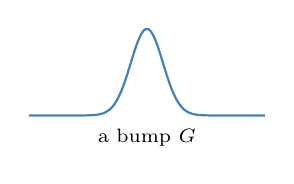
\begin{tikzpicture}[x=0.5cm, y=1cm, every node/.style={font=\scriptsize}]
  \draw[boxframe, thick, domain=-3:3, samples=80, smooth] plot (\x, {1.1*exp(-3*\x*\x)});
  \node[below] at (0,-0.05) {a bump $G$};
\end{tikzpicture}

\vspace{4mm}
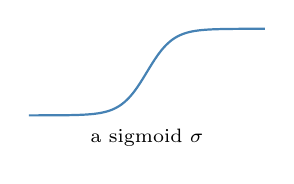
\begin{tikzpicture}[x=0.5cm, y=1cm, every node/.style={font=\scriptsize}]
  \draw[boxframe, thick, domain=-3:3, samples=80, smooth] plot (\x, {1.1/(1+exp(-3*\x))});
  \node[below] at (0,-0.05) {a sigmoid $\sigma$};
\end{tikzpicture}

\vspace{4mm}
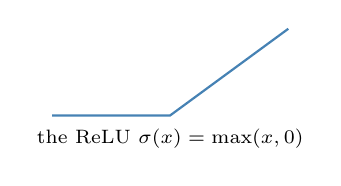
\begin{tikzpicture}[x=0.5cm, y=1cm, every node/.style={font=\scriptsize}]
  \draw[boxframe, thick] (-3,0) -- (0,0) -- (3,1.1);
  \node[below] at (0,-0.05) {the ReLU $\sigma(x)=\max(x,0)$};
\end{tikzpicture}
\end{column}
\end{columns}
\end{frame}


\begin{frame}{Neural networks: shallow versus deep}
\begin{columns}[c]
\begin{column}{0.6\textwidth}
\[
f(x) \sim \sum_{j=1}^{K} \param{\mathbf{w}_j}\, \act{\sigma}(\param{\mathbf{a}_j}\cdot x + \param{b_j})
\]
\centerline{$\Updownarrow$}
\[
\mathbf{x}^{k+1} = \mathbf{x}^k + \ctrl{h}\, \param{\mathbf{w}^k}\, \act{\sigma}(\param{\mathbf{a}^k}\cdot \mathbf{x}^k + \param{b^k})
\]
\centerline{$\Updownarrow$}
\[
\frac{d\mathbf{x}(t)}{dt} = \param{\mathbf{w}(t)}\, \act{\sigma}(\param{\mathbf{a}(t)}\cdot \mathbf{x}(t) + \param{b(t)})
\]
\small
A shallow network is a sum of $K$ neurons; a deep (residual) network composes layers, $k=0,\dots,L$; as the step $\ctrl{h}\to 0$ the layers become the time of a \alert{neural ODE}.
\end{column}
\begin{column}{0.38\textwidth}
\centering
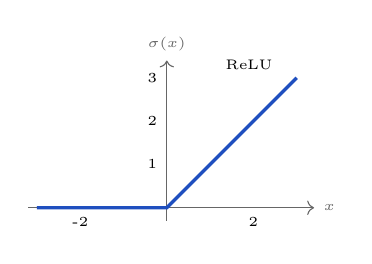
\begin{tikzpicture}[x=0.55cm, y=0.55cm, every node/.style={font=\tiny}]
  \draw[->, black!60] (-3.2,0) -- (3.4,0) node[right] {$x$};
  \draw[->, black!60] (0,-0.3) -- (0,3.4) node[above] {$\sigma(x)$};
  \draw[param, very thick] (-3,0) -- (0,0) -- (3,3);
  \foreach \t in {-2,2} \node[below] at (\t,0) {\t};
  \foreach \t in {1,2,3} \node[left] at (0,\t) {\t};
  \node at (1.9,3.3) {ReLU};
\end{tikzpicture}

\vspace{3mm}
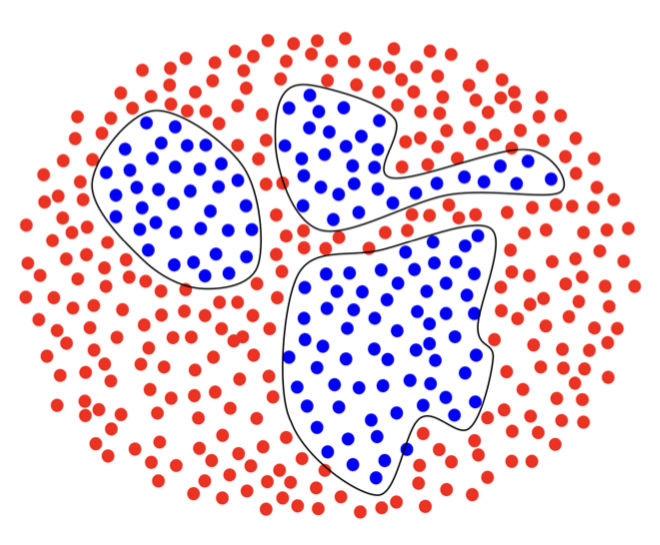
\includegraphics[width=0.9\linewidth]{classification_blobs}
\picnote{Classification: separate the blue from the red points.}
\end{column}
\end{columns}
\end{frame}


\begin{frame}{Supervised learning: computational practice}
\[
\underbrace{\frac{1}{N}\sum_{i=1}^{N} \mathrm{loss}\big(x^i, \ell^i\big)}_{\text{empirical risk} \;:=\; E(x(\cdot))}
\;+\; \alpha \sum_{j=1}^{K} \big\| (\param{\mathbf{a}_j, \mathbf{w}_j, b_j}) \big\|^2
\]
\begin{columns}[c]
\begin{column}{0.55\textwidth}
\centering
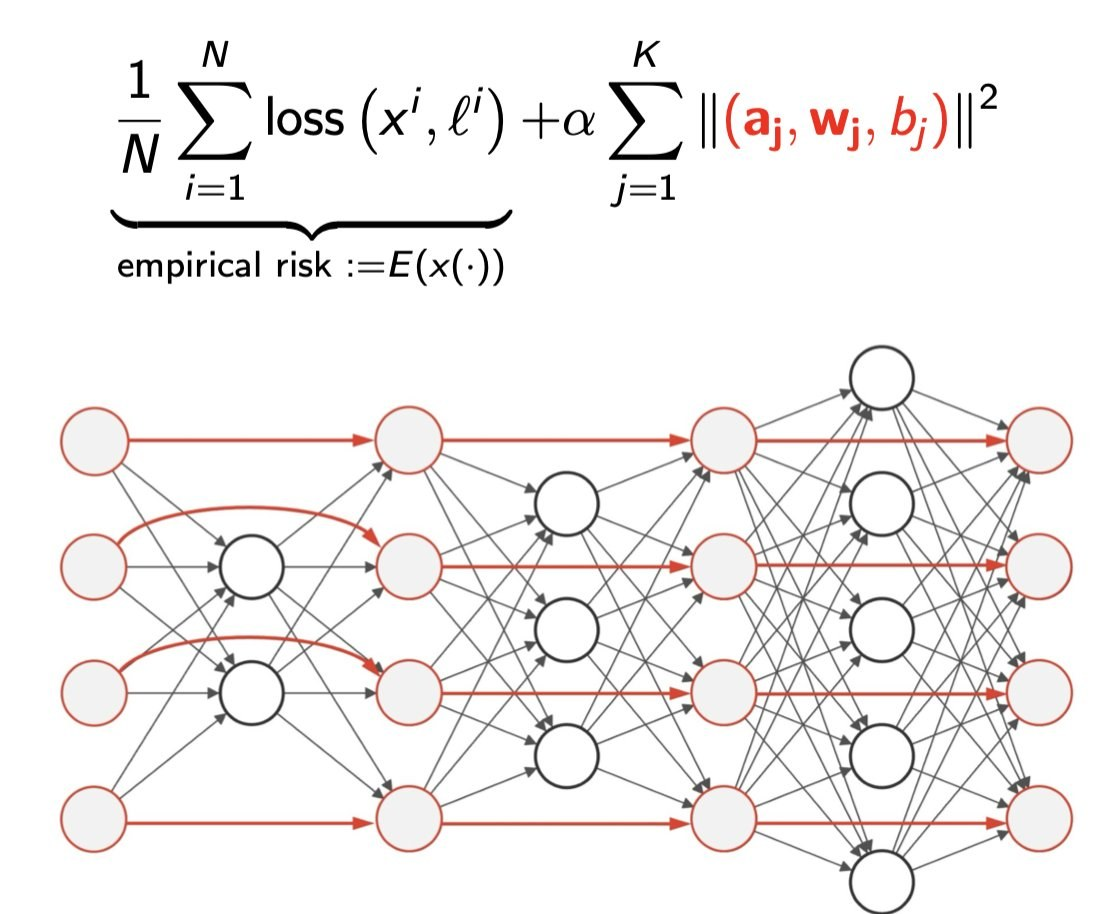
\includegraphics[width=0.96\linewidth]{supervised_learning_network}
\end{column}
\begin{column}{0.43\textwidth}
\small
Given $N$ samples $x^i$ with labels $\ell^i$, choose the parameters $\theta = (\mathbf{a}, \mathbf{b}, \mathbf{w})$ that minimize the empirical risk, plus a penalty on their size.

\medskip
\param{%
\textbf{GPT-3} (2020)\\
175 billion parameters $\theta = (\mathbf{a}, \mathbf{b}, \mathbf{w})$\\
$N = 300$ billion tokens in the training corpus\\
dimension $d = 8{,}192$}
\end{column}
\end{columns}
\end{frame}


\begin{frame}{Least squares}
\begin{columns}[T]
\begin{column}{0.6\textwidth}
\footnotesize
The objective is to adjust the parameters $\beta$ of a model function $f(x,\beta)$ to best fit a data set $(x_i, y_i)$, $i=1,\dots,n$. The fit at a data point is measured by its \alert{residual}
\[
r_i = y_i - f(x_i, \beta).
\]
The least-squares method finds the optimal parameters by minimizing the \alert{sum of squared residuals}
\[
S(\beta) = \sum_{i=1}^{n} r_i^2.
\]
\begin{itemize}
\item In the simplest case $f(x,\beta) = \beta$ and the minimizer is the arithmetic mean of the $y_i$.
\item For a straight line, $f(x,\beta) = \beta_0 + \beta_1 x$: \emph{linear regression}.
\end{itemize}
\scriptsize Legendre (1805) and Gauss (1809). \href{https://en.wikipedia.org/wiki/Least_squares}{Wikipedia: Least squares.}
\end{column}
\begin{column}{0.38\textwidth}
\centering
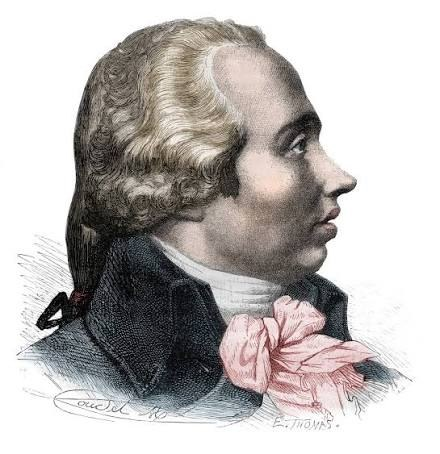
\includegraphics[height=1.9cm]{legendre}\hfill
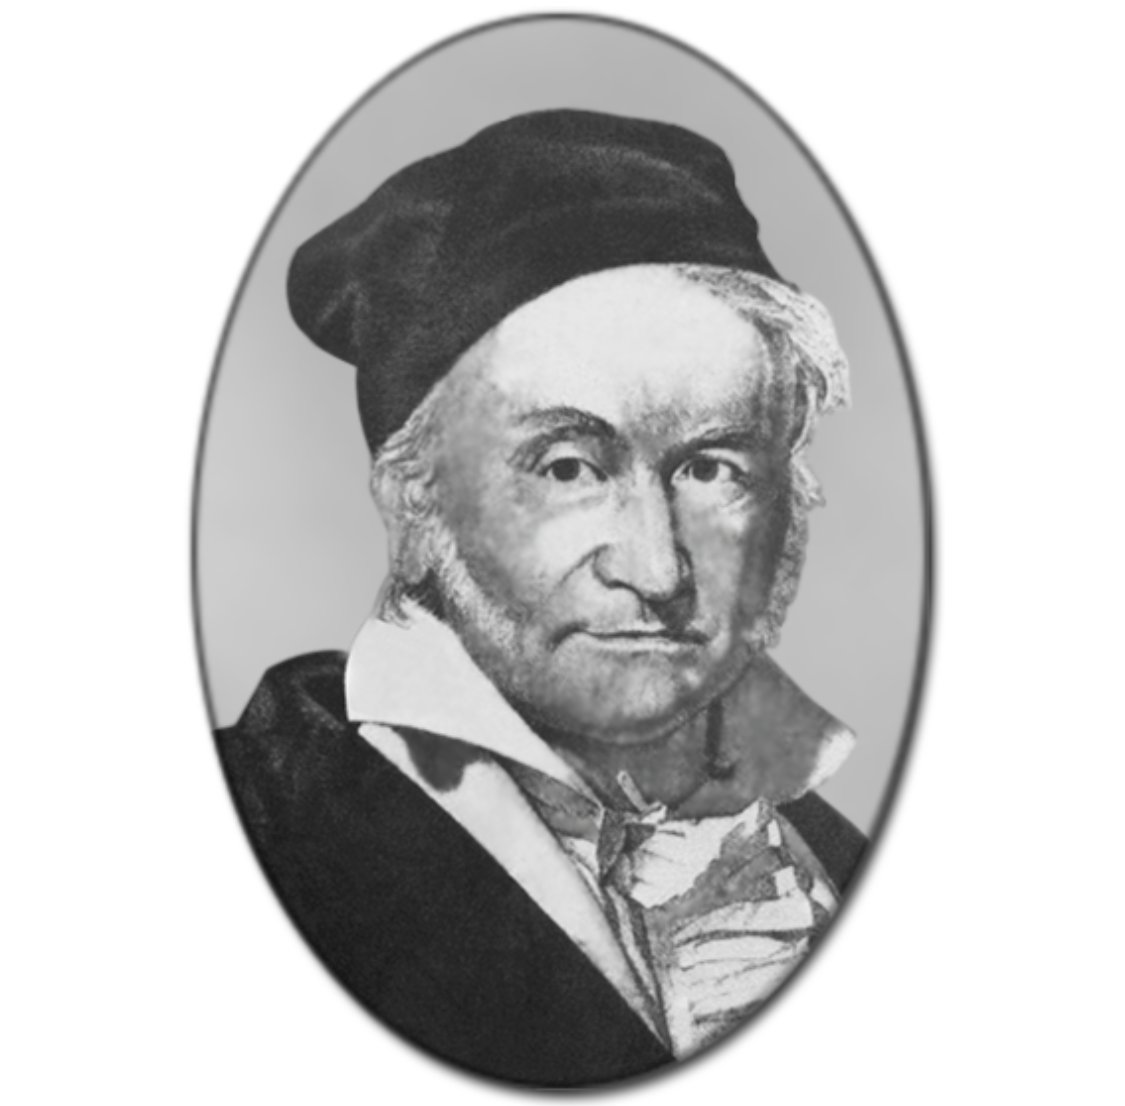
\includegraphics[height=1.9cm]{gauss}
\picnote{A.-M. Legendre \hfill C. F. Gauss}
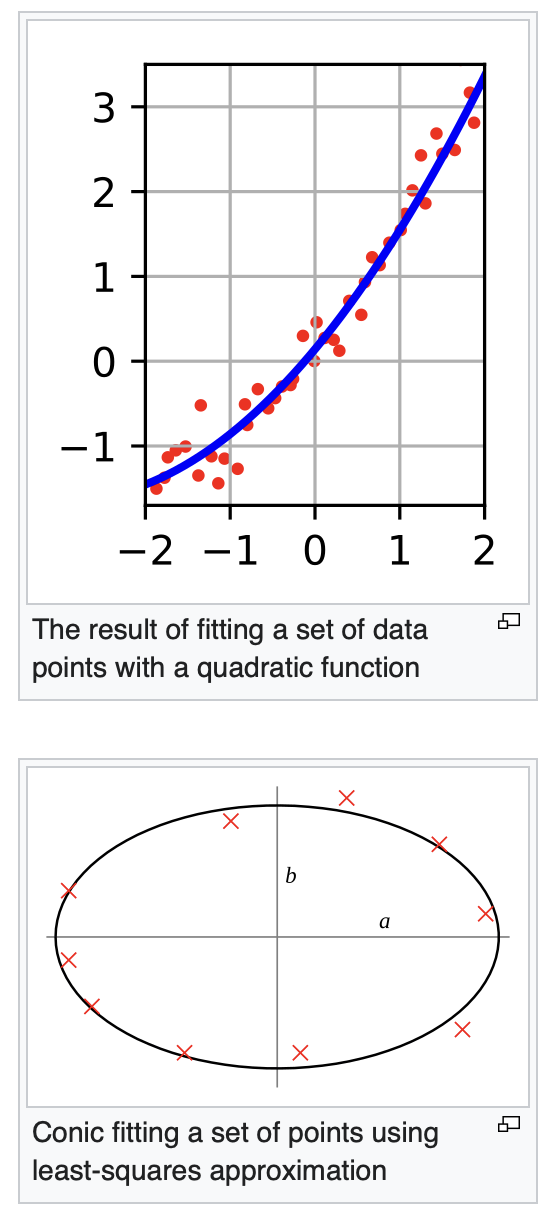
\includegraphics[height=3.4cm]{least_squares_fits}
\end{column}
\end{columns}
\end{frame}


\begin{frame}{Sampling}
\centering
\href{https://en.wikipedia.org/wiki/Sampling_(statistics)}{\fitimg[0.74]{wikipedia_sampling}}
\picnote{A model is trained on a \alert{sample} of the population it should describe. \href{https://en.wikipedia.org/wiki/Sampling_(statistics)}{Wikipedia: Sampling (statistics).}}
\end{frame}


\begin{frame}{The bitter lesson (Rich Sutton, 2019)}
\small
The biggest progress in AI has come from \alert{general methods that leverage computation}, rather than methods that try to incorporate human knowledge.

\medskip
\centering
\href{http://www.incompleteideas.net/IncIdeas/BitterLesson.html}{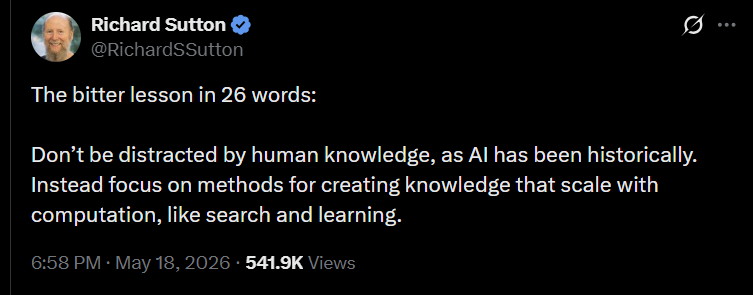
\includegraphics[width=0.9\textwidth]{sutton_bitter_lesson_tweet}}
\picnote{R. Sutton, \href{http://www.incompleteideas.net/IncIdeas/BitterLesson.html}{\emph{The Bitter Lesson}} (2019), and the summary posted by its author in 2026.}
\end{frame}


% =========================================================================
\section{Video material}

\begin{frame}{Video material: 3Blue1Brown, \emph{Neural networks}}
\begin{columns}[T]
\begin{column}{0.48\textwidth}
\videoframe{width=0.92\linewidth}{poster_3b1b_ch1}{https://www.youtube.com/watch?v=aircAruvnKk}{1. But what is a neural network? (19 min)}
\videoframe{width=0.92\linewidth}{poster_3b1b_ch3}{https://www.youtube.com/watch?v=Ilg3gGewQ5U}{3. What is backpropagation really doing? (13 min)}
\end{column}
\begin{column}{0.48\textwidth}
\videoframe{width=0.92\linewidth}{poster_3b1b_ch2}{https://www.youtube.com/watch?v=IHZwWFHWa-w}{2. Gradient descent, how neural networks learn (21 min)}
\videoframe{width=0.92\linewidth}{poster_3b1b_ch4}{https://www.youtube.com/watch?v=tIeHLnjs5U8}{4. Backpropagation calculus (10 min)}
\end{column}
\end{columns}
\end{frame}

\end{document}
